\documentclass[10pt]{article}
\usepackage[utf8]{inputenc}
\usepackage[T1]{fontenc}
\usepackage{amsmath}
\usepackage{amsfonts}
\usepackage{amssymb}
\usepackage[version=4]{mhchem}
\usepackage{stmaryrd}
\usepackage{graphicx}
\usepackage[export]{adjustbox}
\graphicspath{ {./images/} }

\title{Machine Learning Course - CS-433 Regularization: Ridge Regression and Lasso }


\author{Martin Jaggi Last updated on: October 3, 2023}
\date{}


\begin{document}
\maketitle
Oct 4, 2023

credits to Mohammad Emtiyaz Khan \& Rüdiger Urbanke

EPFL

\section*{Motivation}
We have seen that by augmenting the feature vector we can make linear models as powerful as we want. Unfortunately this leads to the problem of overfitting. Regularization is a way to mitigate this undesirable behavior.

We will discuss regularization in the context of linear models, but the same principle applies also to more complex models such as neural nets.

\section*{Regularization}
Through regularization, we can penalize complex models and favor simpler ones:

$$
\min _{\mathbf{w}} \mathcal{L}(\mathbf{w})+\Omega(\mathbf{w})
$$

The second term $\Omega$ is a regularizer, measuring the complexity of the model given by $\mathbf{w}$.

\section*{$L_{2}$-Regularization: Ridge Regression}
The most frequently used regularizer is the standard Euclidean norm $\left(L_{2^{-}}\right.$ norm), that is

$$
\Omega(\mathbf{w})=\lambda\|\mathbf{w}\|_{2}^{2}
$$

where $\|\mathbf{w}\|_{2}^{2}=\sum_{i} w_{i}^{2}$. Here the main effect is that large model weights $w_{i}$ will be penalized (avoided), since we consider them "unlikely", while small ones are ok. When $\mathcal{L}$ is MSE, this is called ridge regression:

$\min _{\mathbf{w}} \frac{1}{2 N} \sum_{n=1}^{N}\left[y_{n}-\mathbf{x}_{n}^{\top} \mathbf{w}\right]^{2}+\lambda\|\mathbf{w}\|_{2}^{2}$

Least squares is a special case of this: set $\lambda:=0$.

\section*{Explicit solution for w: Differ-}
entiating and setting to zero:

$$
\mathbf{w}_{\text {ridge }}^{\star}=\left(\mathbf{X}^{\top} \mathbf{X}+\lambda^{\prime} \mathbf{I}\right)^{-1} \mathbf{X}^{\top} \mathbf{y}
$$

(here for simpler notation $\frac{\lambda^{\prime}}{2 N}=\lambda$ )

\section*{Ridge Regression to Fight III-Conditioning}
The eigenvalues of $\left(\mathbf{X}^{\top} \mathbf{X}+\lambda^{\prime} \mathbf{I}\right)$ are all at least $\lambda^{\prime}$ and so the inverse always exists. This is also referred to as lifting the eigenvalues.

Proof: Write the Eigenvalue decomposition of $\mathbf{X}^{\top} \mathbf{X}$ as $\mathbf{U S U}^{\top}$. We then have

$$
\begin{aligned}
\mathbf{X}^{\top} \mathbf{X}+\lambda^{\prime} \mathbf{I} & =\mathbf{U S} \mathbf{U}^{\top}+\lambda^{\prime} \mathbf{U I U}^{\top} \\
& =\mathbf{U}\left[\mathbf{S}+\lambda^{\prime} \mathbf{I}\right] \mathbf{U}^{\top}
\end{aligned}
$$

We see now that every Eigenvalue is "lifted" by an amount $\lambda^{\prime}$.

Here is an alternative proof. Recall that for a symmetric matrix $\mathbf{A}$ we can also compute eigenvalues by looking at the so-called Rayleigh ratio,

$$
R(\mathbf{A}, \mathbf{v})=\frac{\mathbf{v}^{\top} \mathbf{A} \mathbf{v}}{\mathbf{v}^{\top} \mathbf{v}}
$$

Note that if $\mathbf{v}$ is an eigenvector with eigenvalue $\lambda$ then the Rayleigh coefficient indeed gives us $\lambda$. We can find the smallest and largest eigenvalue by minimizing and maximizing this coefficient. But note that if we apply this to the symmetric matrix $\mathbf{X}^{\top} \mathbf{X}+\lambda^{\prime} \mathbf{I}$ then for any vector $\mathbf{v}$ we have

$$
\frac{\mathbf{v}^{\top}\left(\mathbf{X}^{\top} \mathbf{X}+\lambda^{\prime} \mathbf{I}\right) \mathbf{v}}{\mathbf{v}^{\top} \mathbf{v}} \geq \frac{\lambda^{\prime} \mathbf{v}^{\top} \mathbf{v}}{\mathbf{v}^{\top} \mathbf{v}}=\lambda^{\prime}
$$

\section*{$L_{1}$-Regularization: The Lasso}
As an alternative measure of the complexity of the model, we can use a different norm. A very important case is the $L_{1}$-norm, leading to $L_{1^{-}}$ regularization. In combination with the MSE cost function, this is known as the Lasso:

$\min _{\mathbf{w}} \frac{1}{2 N} \sum_{n=1}^{N}\left[y_{n}-\mathbf{x}_{n}^{\top} \mathbf{w}\right]^{2}+\lambda\|\mathbf{w}\|_{1}$

where

$$
\|\mathbf{w}\|_{1}:=\sum_{i}\left|w_{i}\right| .
$$

\begin{center}
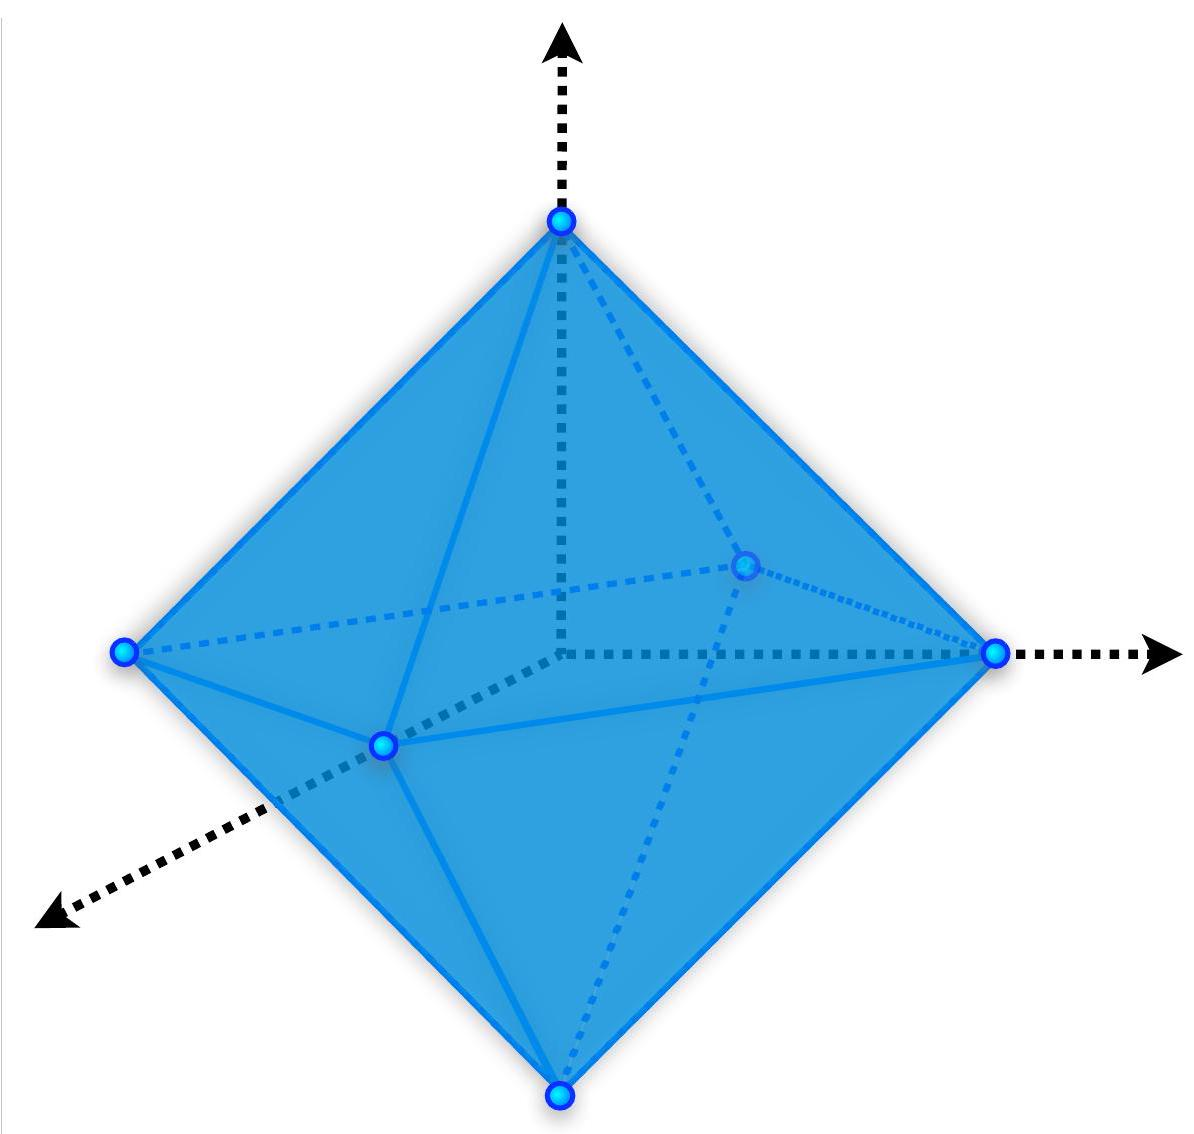
\includegraphics[max width=\textwidth]{2023_12_30_0d309f6e07a388c2ea34g-05}
\end{center}

The figure above shows a "ball" of constant $L_{1}$ norm. To keep things simple assume that $\mathbf{X}^{\top} \mathbf{X}$ is invertible. We claim that in this case the set

$$
\left\{\mathbf{w}:\|\mathbf{y}-\mathbf{X} \mathbf{w}\|^{2}=\alpha\right\}
$$

is an ellipsoid and this ellipsoid simply scales around its origin as we change $\alpha$. We claim that for the $L_{1}$-regularization the optimum solution is likely going to be sparse (only has few non-zero components) compared to the case where we use $L_{2}$-regularization.

Why is this the case? Assume that a genie tells you the $L_{1}$ norm of the optimum solution. Draw the $L_{1}$-ball with that norm value (think of $2 \mathrm{D}$ to visualize it). So now you know that the optimal point is somewhere on the surface of this "ball". Further you know that there are ellipsoids, all with the same mean and rotation that describes the equal error surfaces incurred by the first term. The optimum solution is where the "smallest" of these ellipsoids just touches the $L_{1}$-ball. Due to the geometry of this ball this point is more likely to be on one of the "corner" points. In turn, sparsity is desirable, since it leads to a "simple" model.

How do we see the claim that (1) describes and ellipsoid? First look at $\alpha=\|\mathbf{X w}\|^{2}=\mathbf{w}^{\top} \mathbf{X}^{\top} \mathbf{X w}$. This is a quadratic form. Let $\mathbf{A}=\mathbf{X}^{\top} \mathbf{X}$. Note that $\mathbf{A}$ is a symmetric matrix and by assumption it has full rank. If $\mathbf{A}$ is a diagonal matrix with strictly positive elements $a_{i}$ along the diagonal then this describes the equation

$$
\sum_{i} a_{i} \mathbf{w}_{i}^{2}=\alpha
$$

which is indeed the equation for an ellipsoid. In the general case, $\mathbf{A}$ can be written as (using the SVD) $\mathbf{A}=\mathbf{U B U}^{T}$, where $\mathbf{B}$ is a diagonal matrix with strictly positive entries. This then corresponds to an ellipsoid with rotated axes. If we now look at $\alpha=\|\mathbf{y}-\mathbf{X} \mathbf{w}\|^{2}$, where $\mathbf{y}$ is in the column space of $\mathbf{X}$ then we can write it as $\alpha=\left\|\mathbf{X}\left(\mathbf{w}_{0}-\mathbf{w}\right)\right\|^{2}$ for a suitable chosen $\mathbf{w}_{0}$ and so this corresponds to a shifted ellipsoid. Finally, for the general case, write $\mathbf{y}$ as $\mathbf{y}=\mathbf{y}_{\|}+$ $\mathbf{y}_{\perp}$, where $\mathbf{y}_{\|}$is the component of $\mathbf{y}$ that lies in the subspace spanned by the columns of $\mathbf{X}$ and $\mathbf{y}_{\perp}$ is the component that
is orthogonal. In this case

$$
\begin{aligned}
\alpha & =\|\mathbf{y}-\mathbf{X} \mathbf{w}\|^{2} \\
& =\left\|\mathbf{y}_{\|}+\mathbf{y}_{\perp}-\mathbf{X} \mathbf{w}\right\|^{2} \\
& =\left\|\mathbf{y}_{\perp}\right\|^{2}+\left\|\mathbf{y}_{\|}-\mathbf{X} \mathbf{w}\right\|^{2} \\
& =\left\|\mathbf{y}_{\perp}\right\|^{2}+\left\|\mathbf{X}\left(\mathbf{w}_{0}-\mathbf{w}\right)\right\|^{2} .
\end{aligned}
$$

Hence this is then equivalent to the equation $\left\|\mathbf{X}\left(\mathbf{w}_{0}-\mathbf{w}\right)\right\|^{2}=$ $\alpha-\left\|\mathbf{y}_{\perp}\right\|^{2}$, proving the claim. From this we also see that if $\mathbf{X}^{\top} \mathbf{X}$ is not full rank then what we get is not an ellipsoid but a cylinder with an ellipsoidal cross-section.

\section*{Additional Notes}
\section*{Other Types of Regularization}
Popular methods such as shrinkage, dropout and weight decay (in the context of neural networks), early stopping of the optimization are all different forms of regularization.

Another view of regularization: The ridge regression formulation we have seen above is similar to the following constrained problem (for some $\tau>0)$.

$$
\min _{\mathbf{w}} \frac{1}{2 N} \sum_{n=1}^{N}\left(y_{n}-\mathbf{x}_{n}^{\top} \mathbf{w}\right)^{2}, \quad \text { such that }\|\mathbf{w}\|_{2}^{2} \leq \tau
$$

The following picture illustrates this.

\begin{center}
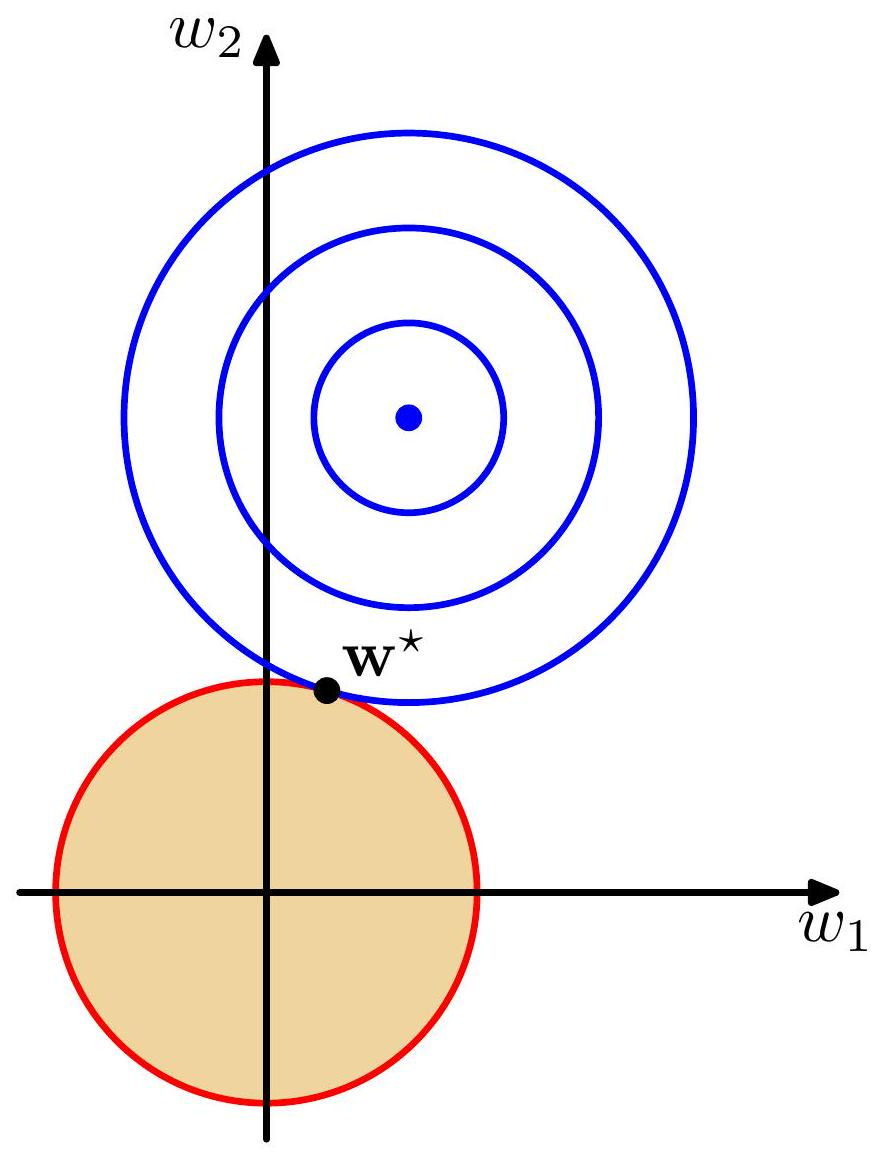
\includegraphics[max width=\textwidth]{2023_12_30_0d309f6e07a388c2ea34g-09}
\end{center}

Figure 1: Geometric interpretation of Ridge Regression. Blue lines indicating the level sets of the MSE cost function.

For the case of using $L_{1}$ regularization (known as the Lasso, when used with MSE) we analogously consider

$$
\min _{\mathbf{w}} \frac{1}{2 N} \sum_{n=1}^{N}\left(y_{n}-\mathbf{x}_{n}^{\top} \mathbf{w}\right)^{2}, \quad \text { such that }\|\mathbf{w}\|_{1} \leq \tau
$$

This forces some of the elements of $\mathbf{w}$ to be strictly 0 and therefore enforces sparsity in the model (some features will not be used since their coefficients are zero).

\begin{itemize}
  \item Why does $L_{1}$ regularizer enforce sparsity? Hint: Draw the picture similar to above, and locate the optimal solution.
  \item Why is it good to have sparsity in the model? Is it going to be better than least-squares? When and why?
\end{itemize}

\section*{Ridge Regression as MAP estimator}
Recall that classic least-squares linear regression can be interpreted as the maximum likelihood estimator:

$$
\begin{aligned}
& \mathbf{w}_{\mathrm{lse}} \stackrel{(a)}{=} \arg \min _{\mathbf{w}}-\log p(\mathbf{y}, \mathbf{X} \mid \mathbf{w}) \\
& \stackrel{(b)}{=} \arg \min _{\mathbf{w}}-\log p(\mathbf{X} \mid \mathbf{w}) p(\mathbf{y} \mid \mathbf{X}, \mathbf{w}) \\
& \stackrel{(c)}{=} \arg \min _{\mathbf{w}}-\log p(\mathbf{X}) p(\mathbf{y} \mid \mathbf{X}, \mathbf{w}) \\
& \stackrel{(d)}{=} \arg \min _{\mathbf{w}} \quad-\log p(\mathbf{y} \mid \mathbf{X}, \mathbf{w}) \\
& \stackrel{(e)}{=} \arg \min _{\mathbf{w}} \quad-\log \left[\prod_{n=1}^{N} p\left(y_{n} \mid \mathbf{x}_{n}, \mathbf{w}\right)\right] \\
& \stackrel{(f)}{=} \arg \min _{\mathbf{w}}-\log \left[\prod_{n=1}^{N} \mathcal{N}\left(y_{n} \mid \mathbf{x}_{n}^{\top} \mathbf{w}, \sigma^{2}\right)\right] \\
& =\arg \min _{\mathbf{w}}-\log \left[\prod_{n=1}^{N} \frac{1}{\sqrt{2 \pi \sigma^{2}}} e^{-\frac{1}{2 \sigma^{2}}\left(y_{n}-\mathbf{x}_{n}^{\top} \mathbf{w}\right)^{2}}\right] \\
& =\arg \min _{\mathbf{w}}-N \log \left(\frac{1}{\sqrt{2 \pi \sigma^{2}}}\right)+\sum_{n=1}^{N} \frac{1}{2 \sigma^{2}}\left(y_{n}-\mathbf{x}_{n}^{\top} \mathbf{w}\right)^{2} \\
& =\arg \min _{\mathbf{w}} \frac{1}{2 \sigma^{2}} \sum_{n=1}^{N}\left(y_{n}-\mathbf{x}_{n}^{\top} \mathbf{w}\right)^{2}
\end{aligned}
$$

In step (a) on the right we wrote down the negative of the log of the likelihood. The maximum likelihood criterion choses that parameter $\mathbf{w}$ that minimizes this quantity (i.e., maximizes the likelihood). In step (b) we factored the likelihood. The usual assumption is that the choice of the input samples $\mathbf{x}_{n}$ does not depend on the model parameter (which only influces the output given the input. Hence, in step (c) we removed the conditioning. Since the factor $p(\mathbf{X})$ does not depend on $\mathbf{w}$, i.e., is a constant wrt to w) we can remove it. This is done in step (d). In step (e) we used the assumption that the samples are iid. In step (f) we then used our assumption that the samples have the form $y_{n}=\mathbf{w}_{n}^{\top} \mathbf{w}+Z_{n}$,
where $Z_{n}$ is a Gaussian noise with mean zero and variance $\sigma_{2}$. The rest is calculus.

Ridge regression has a very similar interpretation. Now we start with the posterior $p(\mathbf{w} \mid \mathbf{X}, \mathbf{y})$ and chose that parameter $\mathbf{w}$ that maximizes this posterior. Hence this is called the maximum-a-posteriori (MAP) estimate. As before, we take the log and add a minus sign and minimize instead. In order to compute the posterior we use Bayes law and we assume that the components of the weight vector are iid Gaussians with mean zero and variance $\frac{1}{\lambda}$.

$$
\begin{aligned}
& \mathbf{w}_{\text {ridge }}=\arg \min _{\mathbf{w}} \quad-\log p(\mathbf{w} \mid \mathbf{X}, \mathbf{y}) \\
& \stackrel{(a)}{=} \arg \min _{\mathbf{w}}-\log \frac{p(\mathbf{y}, \mathbf{X} \mid \mathbf{w}) p(\mathbf{w})}{p(\mathbf{y}, \mathbf{X})} \\
& \stackrel{(b)}{=} \arg \min _{\mathbf{w}}-\log p(\mathbf{y}, \mathbf{X} \mid \mathbf{w}) p(\mathbf{w}) \\
& \stackrel{(c)}{=} \arg \min _{\mathbf{w}} \quad-\log p(\mathbf{y} \mid \mathbf{X}, \mathbf{w}) p(\mathbf{w}) \\
& =\arg \min _{\mathbf{w}}-\log \left[p(\mathbf{w}) \prod_{n=1}^{N} p\left(y_{n} \mid \mathbf{x}_{n}, \mathbf{w}\right)\right] \\
& =\arg \min _{\mathbf{w}}-\log \left[\mathcal{N}\left(\mathbf{w} \mid 0, \frac{1}{\lambda} \mathbf{I}\right) \prod_{n=1}^{N} \mathcal{N}\left(y_{n} \mid \mathbf{x}_{n}^{\top} \mathbf{w}, \sigma^{2}\right)\right] \\
& =\arg \min _{\mathbf{w}}-\log \left[\frac{1}{\left(2 \pi \frac{1}{\lambda}\right)^{D / 2}} e^{-\frac{\lambda}{2}\|\mathbf{w}\|^{2}} \prod_{n=1}^{N} \frac{1}{\sqrt{2 \pi \sigma^{2}}} e^{-\frac{1}{2 \sigma^{2}}\left(y_{n}-\mathbf{x}_{n}^{\top} \mathbf{w}\right)^{2}}\right] \\
& =\arg \min _{\mathbf{w}} \sum_{n=1}^{N} \frac{1}{2 \sigma^{2}}\left(y_{n}-\mathbf{x}_{n}^{\top} \mathbf{w}\right)^{2}+\frac{\lambda}{2}\|\mathbf{w}\|^{2}
\end{aligned}
$$

In step (a) we used Bayes' law. In step (b) and (c) we eliminated quantities that do not depend on $\mathbf{w}$.


\end{document}